\documentclass[a4paper, 12pt]{article}
\title{This is my work in R}
\author{ MyFirstName MyLastName\\OrganizationName\\
         City, ZipCope, \underline{Country}\\
        \url{username@the.rest}}
\date{\today}  %% manually: \date{February 1, 2023} 
\usepackage[natbibapa]{apacite} %% for bibliography
\usepackage{rotating, graphicx} %% for rotating tables
\usepackage{adjustbox} % size of plots and tables
\usepackage{chngcntr}% section numbering
\counterwithin{table}{section}\counterwithin{figure}{section}
\usepackage{Sweave}
\begin{document} % every "begin: needs and "end"
\Sconcordance{concordance:WorkInR_forPrinter.tex:WorkInR_forPrinter.Rnw:%
1 11 1 1 0 8 1 1 5 18 1 1 11 11 1 1 18 16 0 1 3 12 1 1 12 1 2 14 1 1 15 %
23 0 1 2 7 1 1 11 1 2 9 1 1 8 24 0 1 2 9 1 1 9 4 1 1 7 29 0 1 2 17 1 1 %
16 3 1 1 3 1 2 10 1 1 7 1 2 20 1}

\maketitle 
\begin{abstract}
This is an example of an abstract in a paper. This is an example of an abstract in a paper. This is an example of an abstract in a paper. This is an example of an abstract in a paper.This is an example of an abstract in a paper.This is an example of an abstract in a paper.
\end{abstract}

% a chunk hidden (echo=FALSE) with some setup
% chunk has its own name 


\section*{Introduction} % * to unnumber

This is just my intro to my nice paper. This is just my intro to my nice paper.This is just my intro to my nice paper. This is just my intro to my nice paper.This is just my intro to my nice paper. This is just my intro to my nice paper.This is just my intro to my nice paper. This is just my intro to my nice paper.This is just my intro to my nice paper. This is just my intro to my nice paper.This is just my intro to my nice paper. This is just my intro to my nice paper.

This is just my intro to my nice paper. This is just my intro to my nice paper.This is just my intro to my nice paper. This is just my intro to my nice paper.This is just my intro to my nice paper. This is just my intro to my nice paper.This is just my intro to my nice paper. This is just my intro to my nice paper.


\section{Exploring Tables}\label{explo-tables} % label for crossref

%footnote coming
Another section. I will use a footnot now \footnote{This is a footnote.}. I will soon use cross-ref.I will soon use cross-ref.I will soon use cross-ref.I will soon use cross-ref. I will soon use cross-ref. I will soon use cross-ref.I will soon use cross-ref.I will soon use cross-ref.I will soon use cross-ref.I will soon use cross-ref. I will soon use cross-ref. I will soon use cross-ref.
%cross-ref coming

%cross-ref coming
I will soon use cross-ref.I will soon use cross-ref: as we see in Section \ref{catexplor}.



\subsection{Exploring Categorical Data}\label{catexplor}

Here, I continue doing this nice work, I hope you like it and read it. It has been a very hard work.Here, I continue doing this nice work, I hope you like it and read it. It has been a very hard work.Here, I continue doing this nice work, I hope you like it and read it. It has been a very hard work.Here, I continue doing this nice work, I hope you like it and read it. It has been a very hard work.Here, I continue doing this nice work, I hope you like it and read it. It has been a very hard work.Here, I continue doing this nice work, I hope you like it and read it. It has been a very hard work.

I hope you like it and read it. It has been a very hard work.Here, I continue doing this nice work, I hope you like it and read it. It has been a very hard work.Here, I continue doing this nice work, I hope you like it and read it. It has been a very hard work.Here, I continue doing this nice work, I hope you like it and read it. It has been a very hard work.Here, I continue doing this nice work, I hope you like it and read it. It has been a very hard work.

You can see the statistics of a categorical variable in Table \ref{catexploreTable}.

%the chunk name is NOT used in cross-ref for table.
%Table is created and displayed.

\begin{table}[!h]

\caption{This is a table\label{catexploreTable}}
\centering
\begin{tabular}[t]{l|r|r|r}
\hline
Democracy Level & count & pct & pct\_cumm\\
\hline
Authoritarian & 57 & 36.08 & 36.08\\
\hline
Hybrid regime & 32 & 20.25 & 56.33\\
\hline
Flawed democracy & 50 & 31.65 & 87.97\\
\hline
Full democracy & 19 & 12.03 & 100.00\\
\hline
\end{tabular}
\end{table}

%%%%%%

You can see this variable plotted in Figure \ref{catBarplot} on page \pageref{catBarplot}.

% NO need for figure caption in chunk header.
% Object will be created BUT NOT plotted
% the chunk name IS NOT used in cross-ref for figure

\begin{figure}[h]
\centering
\begin{adjustbox}{width=7cm,height=5cm} %resize
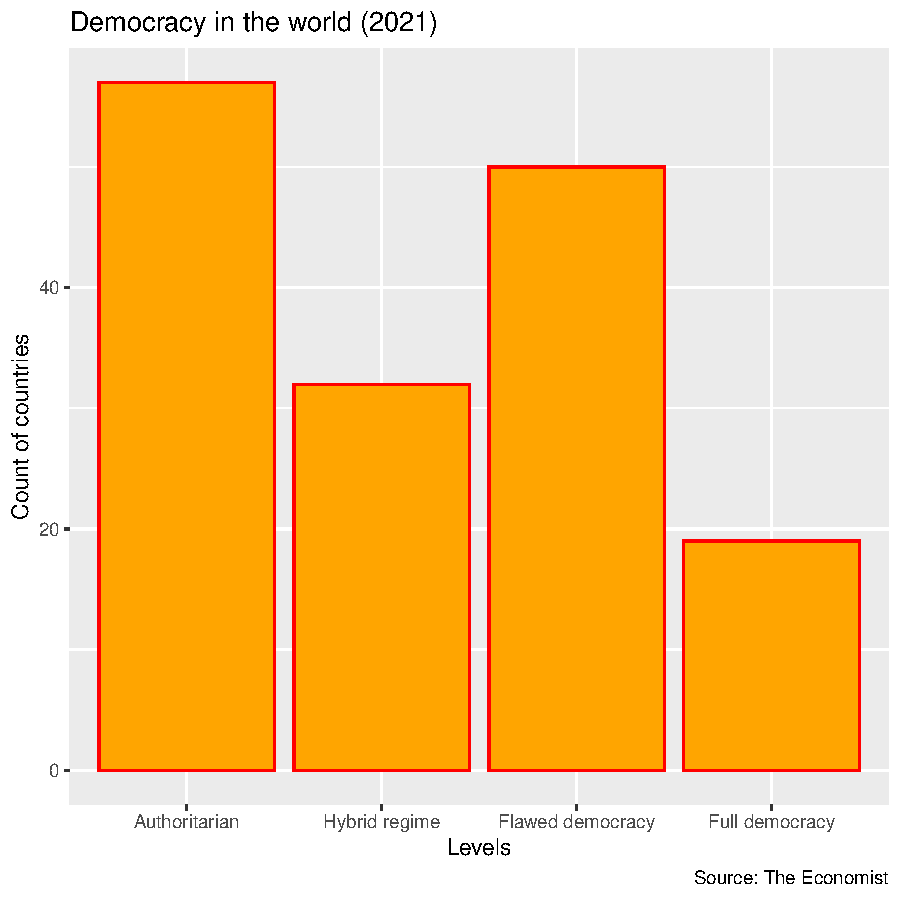
\includegraphics{WorkInR_forPrinter-catBarplot}
\end{adjustbox}
\caption{Press Freedom Index in the World}  %title
\label{catBarplot} % for cross-ref
\end{figure}



\subsection{Exploring Numerical Data}\label{numexplo}

Here, I continue doing this nice work, I hope you like it and read it. It has been a very hard work.Here, I continue doing this nice work, I hope you like it and read it. It has been a very hard work.Here, I continue doing this nice work, I hope you like it and read it. It has been a very hard work.Here, I continue doing this nice work, I hope you like it and read it. It has been a very hard work.Here, I continue doing this nice work, I hope you like it and read it. It has been a very hard work.Here, I continue doing this nice work, I hope you like it and read it. It has been a very hard work.Here, I continue doing this nice work, I hope you like it and read it. It has been a very hard work.Here, I continue doing this nice work, I hope you like it and read it. It has been a very hard work.Here, I continue doing this nice work, I hope you like it and read it. It has been a very hard work.

Here, I continue doing this nice work, I hope you like it and read it. It has been a very hard work.Here, I continue doing this nice work, I hope you like it and read it. It has been a very hard work.Here, I continue doing this nice work, I hope you like it and read it. It has been a very hard work.Here, I continue doing this nice work, I hope you like it and read it. It has been a very hard work.Here, I continue doing this nice work, I hope you like it and read it. It has been a very hard work.Here, I continue doing this nice work, I hope you like it and read it. It has been a very hard work.Here, I continue doing this nice work, I hope you like it and read it. It has been a very hard work.Here, I continue doing this nice work, I hope you like it and read it. It has been a very hard work.Here, I continue doing this nice work, I hope you like it and read it. It has been a very hard work.

Here, I continue doing this nice work, I hope you like it and read it. It has been a very hard work.Here, I continue doing this nice work, I hope you like it and read it. It has been a very hard work.

% Table created by stargazer v.5.2.3 by Marek Hlavac, Social Policy Institute. E-mail: marek.hlavac at gmail.com
% Date and time: Mon, Feb 13, 2023 - 1:39:23 PM
\begin{table}[!htbp] \centering 
  \caption{Stat summary for numeric vars} 
  \label{summaryNumeric} 
\scriptsize 
\begin{tabular}{@{\extracolsep{5pt}}lccccccc} 
\\[-1.8ex]\hline 
\hline \\[-1.8ex] 
Statistic & \multicolumn{1}{c}{N} & \multicolumn{1}{c}{Mean} & \multicolumn{1}{c}{St. Dev.} & \multicolumn{1}{c}{Min} & \multicolumn{1}{c}{Pctl(25)} & \multicolumn{1}{c}{Pctl(75)} & \multicolumn{1}{c}{Max} \\ 
\hline \\[-1.8ex] 
HumanDevelopmentIndex & 158 & 0.72 & 0.16 & 0.39 & 0.59 & 0.85 & 0.96 \\ 
LifeExpectancyAtBirth & 158 & 71.17 & 7.89 & 52.53 & 65.05 & 76.82 & 85.47 \\ 
ExpectedYearsOfSchooling & 158 & 13.60 & 2.98 & 6.96 & 11.51 & 15.70 & 21.05 \\ 
MeanYearsOfSchooling & 158 & 8.96 & 3.32 & 2.11 & 6.05 & 11.64 & 14.09 \\ 
GrossNationalIncomePerCapita & 158 & 20,126.60 & 20,390.02 & 731.79 & 4,552.38 & 30,106.04 & 90,918.64 \\ 
Overallscore & 158 & 5.26 & 2.29 & 0.32 & 3.21 & 7.00 & 9.75 \\ 
Electoralprocessandpluralism & 158 & 5.60 & 3.81 & 0.00 & 1.44 & 9.17 & 10.00 \\ 
Functioningofgovernment & 158 & 4.58 & 2.58 & 0.00 & 2.50 & 6.43 & 9.64 \\ 
Politicalparticipation & 158 & 5.40 & 1.95 & 0.00 & 3.89 & 6.67 & 10.00 \\ 
Politicalculture & 158 & 5.35 & 1.82 & 1.25 & 3.75 & 6.25 & 10.00 \\ 
Civilliberties & 158 & 5.37 & 2.66 & 0.00 & 3.24 & 7.65 & 9.71 \\ 
\hline \\[-1.8ex] 
\end{tabular} 
\end{table} 
% Use of R object inline
In the Table \ref{summaryNumeric}, you realize that the mean of HDI is {\bf0.72}. It would be good to see a boxplot, check Figure \ref{numBoxplot} below.


\begin{figure}[h]
\centering
\begin{adjustbox}{width=12cm,height=8.5cm,clip,trim=0cm 0.5cm 0cm 0cm} 
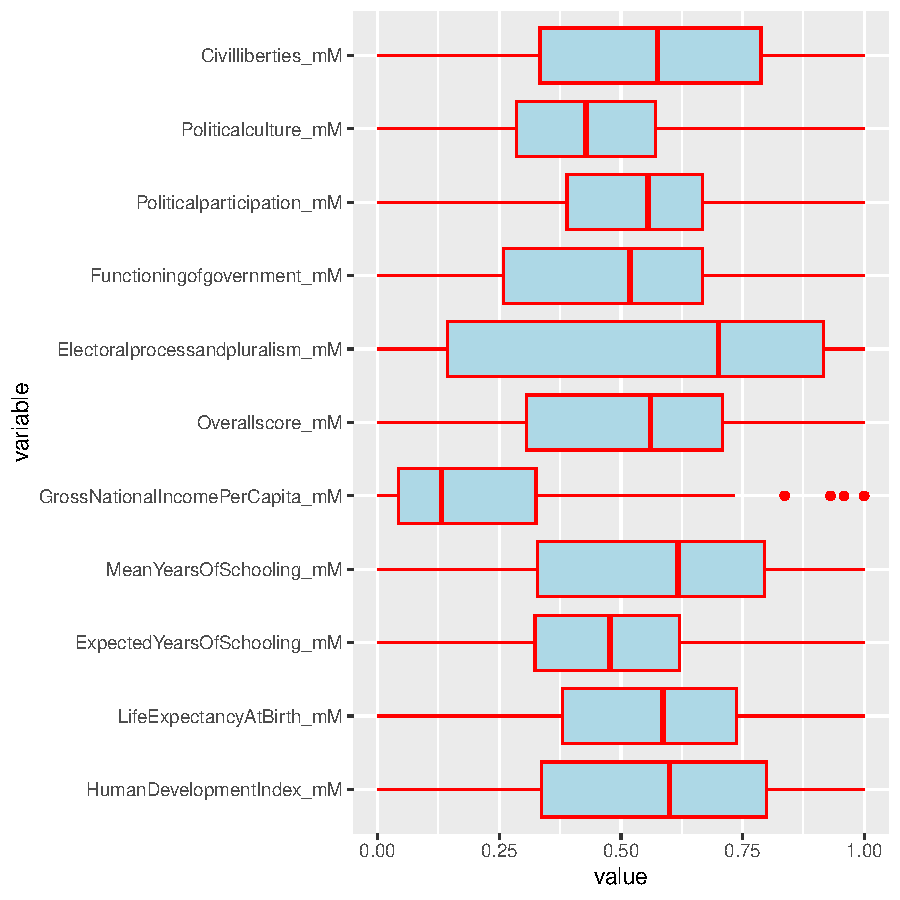
\includegraphics{WorkInR_forPrinter-numBoxplot}
\end{adjustbox}
\caption{Money spent per country on Military stuff}  
\label{numBoxplot} 
\end{figure}

%%%%% A citation: author(year)
Boxplots were introduced by \citet{tukey_exploratory_1977}. You can also flip the Table \ref{summaryNumeric}, as shown in Table \ref{summaryNumeric-flip}.



% Table created by stargazer v.5.2.3 by Marek Hlavac, Social Policy Institute. E-mail: marek.hlavac at gmail.com
% Date and time: Mon, Feb 13, 2023 - 1:39:24 PM
% Requires LaTeX packages: rotating 
\begin{sidewaystable}[!htbp] \centering 
  \caption{Stat summary for numeric vars (flipped)} 
  \label{summaryNumeric-flip} 
\scriptsize 
\begin{tabular}{@{\extracolsep{5pt}}lccccccc} 
\\[-1.8ex]\hline 
\hline \\[-1.8ex] 
Statistic & \multicolumn{1}{c}{N} & \multicolumn{1}{c}{Mean} & \multicolumn{1}{c}{St. Dev.} & \multicolumn{1}{c}{Min} & \multicolumn{1}{c}{Pctl(25)} & \multicolumn{1}{c}{Pctl(75)} & \multicolumn{1}{c}{Max} \\ 
\hline \\[-1.8ex] 
HumanDevelopmentIndex & 158 & 0.72 & 0.16 & 0.39 & 0.59 & 0.85 & 0.96 \\ 
LifeExpectancyAtBirth & 158 & 71.17 & 7.89 & 52.53 & 65.05 & 76.82 & 85.47 \\ 
ExpectedYearsOfSchooling & 158 & 13.60 & 2.98 & 6.96 & 11.51 & 15.70 & 21.05 \\ 
MeanYearsOfSchooling & 158 & 8.96 & 3.32 & 2.11 & 6.05 & 11.64 & 14.09 \\ 
GrossNationalIncomePerCapita & 158 & 20,126.60 & 20,390.02 & 731.79 & 4,552.38 & 30,106.04 & 90,918.64 \\ 
Overallscore & 158 & 5.26 & 2.29 & 0.32 & 3.21 & 7.00 & 9.75 \\ 
Electoralprocessandpluralism & 158 & 5.60 & 3.81 & 0.00 & 1.44 & 9.17 & 10.00 \\ 
Functioningofgovernment & 158 & 4.58 & 2.58 & 0.00 & 2.50 & 6.43 & 9.64 \\ 
Politicalparticipation & 158 & 5.40 & 1.95 & 0.00 & 3.89 & 6.67 & 10.00 \\ 
Politicalculture & 158 & 5.35 & 1.82 & 1.25 & 3.75 & 6.25 & 10.00 \\ 
Civilliberties & 158 & 5.37 & 2.66 & 0.00 & 3.24 & 7.65 & 9.71 \\ 
\hline \\[-1.8ex] 
\end{tabular} 
\end{sidewaystable} 
\pagebreak



%%%%
\section{My Regression}\label{regre}

Several times we need regression. This is a nice summary for two regressions, as shown in Table \ref{regs1}:






% Table created by stargazer v.5.2.3 by Marek Hlavac, Social Policy Institute. E-mail: marek.hlavac at gmail.com
% Date and time: Mon, Feb 13, 2023 - 1:39:24 PM
\begin{table}[!htbp] \centering 
  \caption{Models for HDI} 
  \label{regs1} 
\begin{tabular}{@{\extracolsep{5pt}}lcc} 
\\[-1.8ex]\hline 
\hline \\[-1.8ex] 
 & \multicolumn{2}{c}{\textit{Dependent variable:}} \\ 
\cline{2-3} 
\\[-1.8ex] & \multicolumn{2}{c}{Human Development} \\ 
\\[-1.8ex] & (1) & (2)\\ 
\hline \\[-1.8ex] 
 Bureaucracy & 0.042$^{***}$ & 0.036$^{***}$ \\ 
  & (0.003) & (0.005) \\ 
  & & \\ 
 Participation &  & 0.013$^{**}$ \\ 
  &  & (0.006) \\ 
  & & \\ 
 Constant & 0.526$^{***}$ & 0.488$^{***}$ \\ 
  & (0.018) & (0.026) \\ 
  & & \\ 
\hline \\[-1.8ex] 
Observations & 158 & 158 \\ 
Log Likelihood & 121.396 & 123.419 \\ 
Akaike Inf. Crit. & $-$238.792 & $-$240.837 \\ 
\hline 
\hline \\[-1.8ex] 
\textit{Note:}  & \multicolumn{2}{r}{$^{*}$p$<$0.1; $^{**}$p$<$0.05; $^{***}$p$<$0.01} \\ 
\end{tabular} 
\end{table} 
I hope you like what you see in the Table \ref{regs1}. You can learn more on regression in 
other book \citep[150-160]{petrie_introduction_2016}

%%%%


\section{Other plots}\label{otherPlots}


\subsection{A map}\label{mapPlot}

Let me show a nice map.Let me show a nice map.Let me show a nice map.Let me show a nice map.Let me show a nice map.Let me show a nice map.Let me show a nice map.Let me show a nice map.Let me show a nice map.Let me show a nice map.Let me show a nice map.Let me show a nice map.

Let me show a nice map.Let me show a nice map.Let me show a nice map.Let me show a nice map.Let me show a nice map.Let me show a nice map.Let me show a nice map.Let me show a nice map.Let me show a nice map.Let me show a nice map.Let me show a nice map.Let me show a nice map.

Let me show a nice map.Let me show a nice map.Let me show a nice map.Let me show a nice map.Let me show a nice map.Let me show a nice map.Let me show a nice map.Let me show a nice map.Let me show a nice map.Let me show a nice map.Let me show a nice map.Let me show a nice map in Figure \ref{plot-cityMap}.


\begin{figure}[h]
\centering
\begin{adjustbox}{width=10cm,height=10cm} 
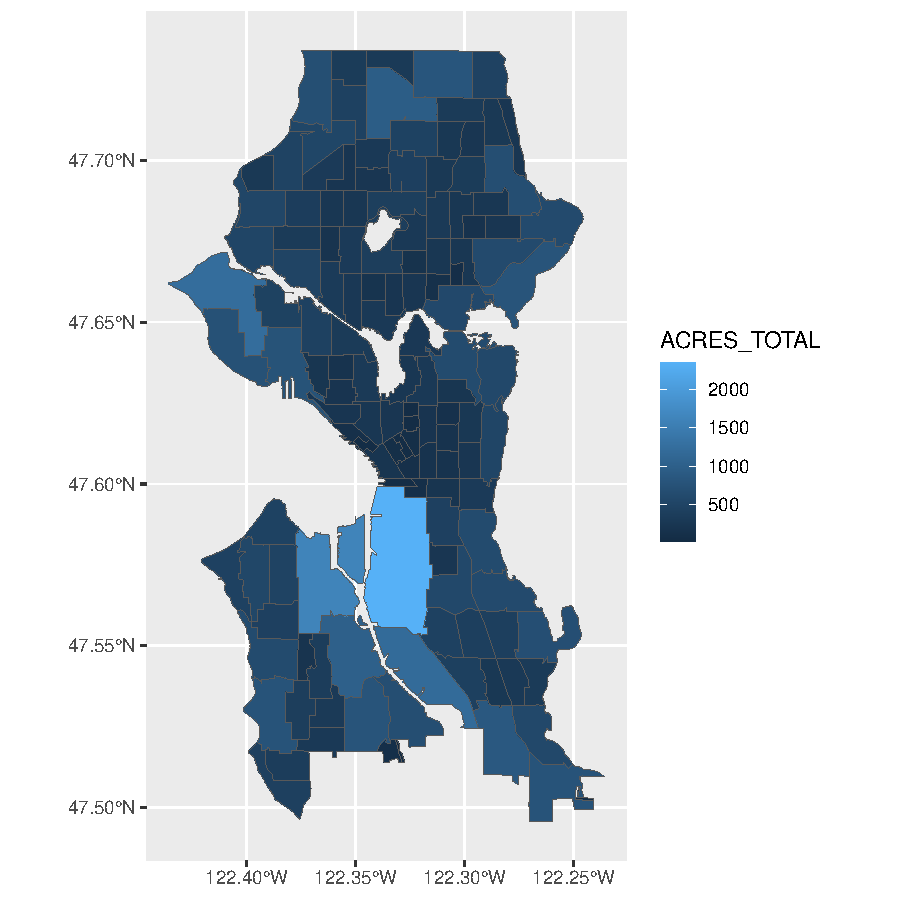
\includegraphics{WorkInR_forPrinter-plot-cityMap}
\end{adjustbox}
\caption{Plot numeric colums.}  
\label{plot-cityMap} 
\end{figure}

Figure \ref{plot-cityMap} uses only one layer. Let's add another layer in the next map. Here, I continue doing this nice work, I hope you like it and read it. It has been a very hard work.Here, I continue doing this nice work, I hope you like it and read it. It has been a very hard work.Here, I continue doing this nice work, I hope you like it and read it. It has been a very hard work.Here, I continue doing this nice work, I hope you like it and read it.  Here, I continue doing this nice work, I hope you like it and read it. It has been a very hard work.Here, I continue doing this nice work, I hope you like it and read it. It has been a very hard work.Here, I continue doing this nice work, I hope you like it and read it. It has been a very hard work.Here, I continue doing this nice work, I hope you like it and read it.


\begin{figure}[h]
\centering
\begin{adjustbox}{width=10cm,height=10cm} 
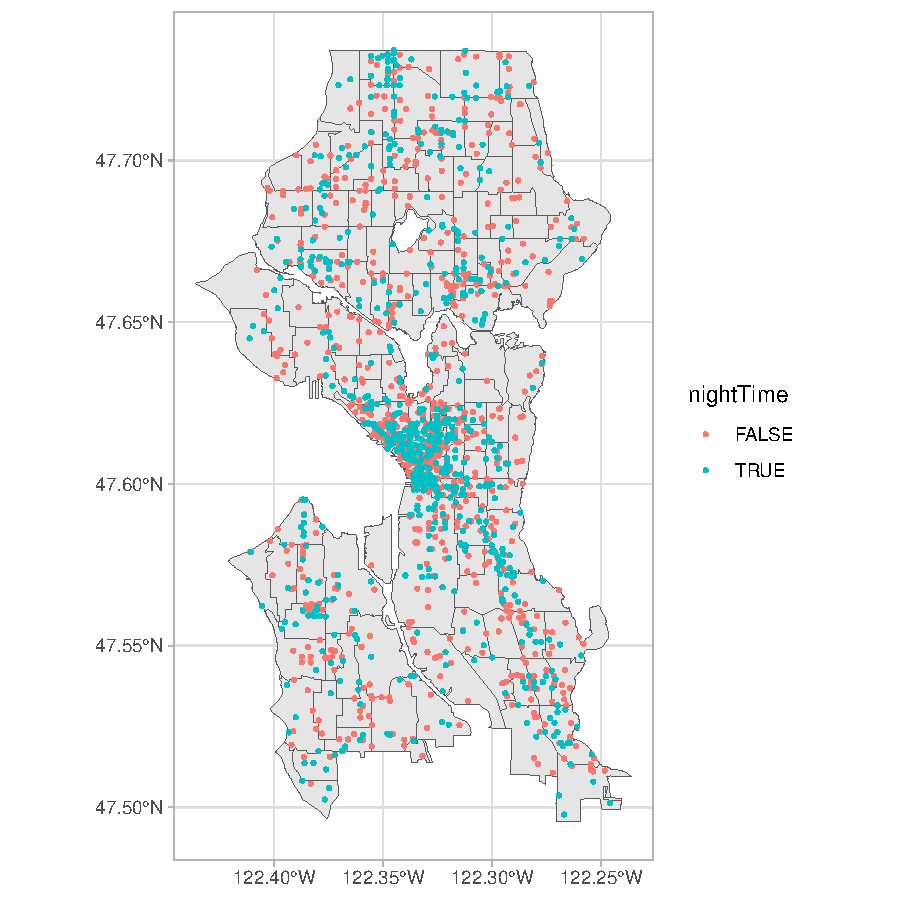
\includegraphics{WorkInR_forPrinter-plot-911Map}
\end{adjustbox}
\caption{Calls to 911 by time of day.}  
\label{plot-911Map} 
\end{figure}

You can see that Figure \ref{plot-911Map} actually uses one map on top of the other. 
Here, I continue doing this nice work, I hope you like it and read it. It has been a very hard work.Here, I continue doing this nice work, I hope you like it and read it. It has been a very hard work.Here, I continue doing this nice work, I hope you like it and read it. It has been a very hard work.Here, I continue doing this nice work, I hope you like it and read it. 

%% more than one author in a citation
Review other authors 
(\citealp[120-160]{brunsdon_introduction_2015};
\citealp[also, see][]{camara_spatial_nodate}) to know more.

\newpage

%%%%% adding bibliography
\bibliographystyle{apacite} %%style
%\renewcommand{\refname}{Bibliography}
\bibliography{Bib_winterschool} %% filename
\end{document} %% nothing after here

